\documentclass[twoside]{book}

% Packages required by doxygen
\usepackage{fixltx2e}
\usepackage{calc}
\usepackage{doxygen}
\usepackage[export]{adjustbox} % also loads graphicx
\usepackage{graphicx}
\usepackage[utf8]{inputenc}
\usepackage{makeidx}
\usepackage{multicol}
\usepackage{multirow}
\PassOptionsToPackage{warn}{textcomp}
\usepackage{textcomp}
\usepackage[nointegrals]{wasysym}
\usepackage[table]{xcolor}

% Font selection
\usepackage[T1]{fontenc}
\usepackage[scaled=.90]{helvet}
\usepackage{courier}
\usepackage{amssymb}
\usepackage{sectsty}
\renewcommand{\familydefault}{\sfdefault}
\allsectionsfont{%
  \fontseries{bc}\selectfont%
  \color{darkgray}%
}
\renewcommand{\DoxyLabelFont}{%
  \fontseries{bc}\selectfont%
  \color{darkgray}%
}
\newcommand{\+}{\discretionary{\mbox{\scriptsize$\hookleftarrow$}}{}{}}

% Page & text layout
\usepackage{geometry}
\geometry{%
  a4paper,%
  top=2.5cm,%
  bottom=2.5cm,%
  left=2.5cm,%
  right=2.5cm%
}
\tolerance=750
\hfuzz=15pt
\hbadness=750
\setlength{\emergencystretch}{15pt}
\setlength{\parindent}{0cm}
\setlength{\parskip}{0.2cm}
\makeatletter
\renewcommand{\paragraph}{%
  \@startsection{paragraph}{4}{0ex}{-1.0ex}{1.0ex}{%
    \normalfont\normalsize\bfseries\SS@parafont%
  }%
}
\renewcommand{\subparagraph}{%
  \@startsection{subparagraph}{5}{0ex}{-1.0ex}{1.0ex}{%
    \normalfont\normalsize\bfseries\SS@subparafont%
  }%
}
\makeatother

% Headers & footers
\usepackage{fancyhdr}
\pagestyle{fancyplain}
\fancyhead[LE]{\fancyplain{}{\bfseries\thepage}}
\fancyhead[CE]{\fancyplain{}{}}
\fancyhead[RE]{\fancyplain{}{\bfseries\leftmark}}
\fancyhead[LO]{\fancyplain{}{\bfseries\rightmark}}
\fancyhead[CO]{\fancyplain{}{}}
\fancyhead[RO]{\fancyplain{}{\bfseries\thepage}}
\fancyfoot[LE]{\fancyplain{}{}}
\fancyfoot[CE]{\fancyplain{}{}}
\fancyfoot[RE]{\fancyplain{}{\bfseries\scriptsize Generated on Mon Nov 14 2016 04\+:38\+:24 for Equation Calculation Project by Doxygen }}
\fancyfoot[LO]{\fancyplain{}{\bfseries\scriptsize Generated on Mon Nov 14 2016 04\+:38\+:24 for Equation Calculation Project by Doxygen }}
\fancyfoot[CO]{\fancyplain{}{}}
\fancyfoot[RO]{\fancyplain{}{}}
\renewcommand{\footrulewidth}{0.4pt}
\renewcommand{\chaptermark}[1]{%
  \markboth{#1}{}%
}
\renewcommand{\sectionmark}[1]{%
  \markright{\thesection\ #1}%
}

% Indices & bibliography
\usepackage{natbib}
\usepackage[titles]{tocloft}
\setcounter{tocdepth}{3}
\setcounter{secnumdepth}{5}
\makeindex

% Hyperlinks (required, but should be loaded last)
\usepackage{ifpdf}
\ifpdf
  \usepackage[pdftex,pagebackref=true]{hyperref}
\else
  \usepackage[ps2pdf,pagebackref=true]{hyperref}
\fi
\hypersetup{%
  colorlinks=true,%
  linkcolor=blue,%
  citecolor=blue,%
  unicode%
}

% Custom commands
\newcommand{\clearemptydoublepage}{%
  \newpage{\pagestyle{empty}\cleardoublepage}%
}


%===== C O N T E N T S =====

\begin{document}

% Titlepage & ToC
\hypersetup{pageanchor=false,
             bookmarks=true,
             bookmarksnumbered=true,
             pdfencoding=unicode
            }
\pagenumbering{roman}
\begin{titlepage}
\vspace*{7cm}
\begin{center}%
{\Large Equation Calculation Project \\[1ex]\large 2.\+0 }\\
\vspace*{1cm}
{\large Generated by Doxygen 1.8.9.1}\\
\vspace*{0.5cm}
{\small Mon Nov 14 2016 04:38:24}\\
\end{center}
\end{titlepage}
\clearemptydoublepage
\tableofcontents
\clearemptydoublepage
\pagenumbering{arabic}
\hypersetup{pageanchor=true}

%--- Begin generated contents ---
\chapter{Equation Calculation Project}
\label{index}\hypertarget{index}{}\hypertarget{index_intro_sec}{}\section{Introduction}\label{index_intro_sec}
This project is used to demonstrate how to do real documentation and unit testing\hypertarget{index_install_sec}{}\section{Installation}\label{index_install_sec}
\hypertarget{index_step1}{}\subsection{Step 1\+: Set up build folder}\label{index_step1}
If this folder is not present, run the command


\begin{DoxyCode}
1 mkdir build
\end{DoxyCode}


When you have a build folder run


\begin{DoxyCode}
1 cd build
\end{DoxyCode}
\hypertarget{index_step2}{}\subsection{Step 2\+: Build}\label{index_step2}
Run the command


\begin{DoxyCode}
1 cmake .. && make
\end{DoxyCode}
\hypertarget{index_Run}{}\subsection{the program}\label{index_Run}
In order to run the program run this command from the build folder


\begin{DoxyCode}
1 ./code\_quality\_godlike [parameter a] [parameter b]
\end{DoxyCode}


Where parametere a and b are numbers. a can range from 0 to 12. 
\chapter{Hierarchical Index}
\section{Class Hierarchy}
This inheritance list is sorted roughly, but not completely, alphabetically\+:\begin{DoxyCompactList}
\item exception\begin{DoxyCompactList}
\item \contentsline{section}{argument\+\_\+invalid\+\_\+exception}{\pageref{classargument__invalid__exception}}{}
\item \contentsline{section}{negative\+\_\+number\+\_\+exception}{\pageref{classnegative__number__exception}}{}
\item \contentsline{section}{overflow\+\_\+exception}{\pageref{classoverflow__exception}}{}
\end{DoxyCompactList}
\end{DoxyCompactList}

\chapter{Class Index}
\section{Class List}
Here are the classes, structs, unions and interfaces with brief descriptions\+:\begin{DoxyCompactList}
\item\contentsline{section}{\hyperlink{classargument__invalid__exception}{argument\+\_\+invalid\+\_\+exception} \\*Exception invoked by invalid arguments }{\pageref{classargument__invalid__exception}}{}
\item\contentsline{section}{\hyperlink{classnegative__number__exception}{negative\+\_\+number\+\_\+exception} \\*Exception invoked by negative numbers }{\pageref{classnegative__number__exception}}{}
\item\contentsline{section}{\hyperlink{classoverflow__exception}{overflow\+\_\+exception} \\*Exception invoked by integer overflow }{\pageref{classoverflow__exception}}{}
\end{DoxyCompactList}

\chapter{File Index}
\section{File List}
Here is a list of all documented files with brief descriptions\+:\begin{DoxyCompactList}
\item\contentsline{section}{\hyperlink{code__quality__professional_8cpp}{code\+\_\+quality\+\_\+professional.\+cpp} }{\pageref{code__quality__professional_8cpp}}{}
\end{DoxyCompactList}

\chapter{Class Documentation}
\hypertarget{classargument__invalid__exception}{}\section{argument\+\_\+invalid\+\_\+exception Class Reference}
\label{classargument__invalid__exception}\index{argument\+\_\+invalid\+\_\+exception@{argument\+\_\+invalid\+\_\+exception}}


Exception invoked by invalid arguments.  




{\ttfamily \#include $<$exceptions.\+hpp$>$}



Inheritance diagram for argument\+\_\+invalid\+\_\+exception\+:\nopagebreak
\begin{figure}[H]
\begin{center}
\leavevmode
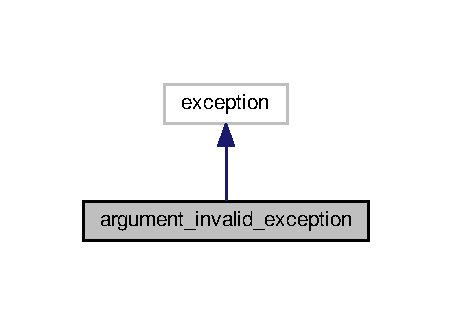
\includegraphics[width=217pt]{classargument__invalid__exception__inherit__graph}
\end{center}
\end{figure}


Collaboration diagram for argument\+\_\+invalid\+\_\+exception\+:\nopagebreak
\begin{figure}[H]
\begin{center}
\leavevmode
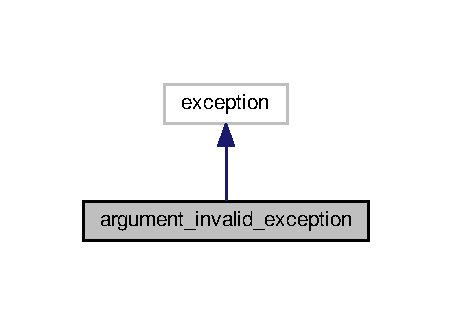
\includegraphics[width=217pt]{classargument__invalid__exception__coll__graph}
\end{center}
\end{figure}
\subsection*{Public Member Functions}
\begin{DoxyCompactItemize}
\item 
virtual const char $\ast$ \hyperlink{classargument__invalid__exception_a83de743404d8fe8de004499488e176ce}{what} () const   throw ()
\begin{DoxyCompactList}\small\item\em Details the problem which invokes the exception. \end{DoxyCompactList}\end{DoxyCompactItemize}
\subsection*{Public Attributes}
\begin{DoxyCompactItemize}
\item 
\hypertarget{classargument__invalid__exception_af349d470216344fd7f5f4017e6eb2a7a}{}char $\ast$ \hyperlink{classargument__invalid__exception_af349d470216344fd7f5f4017e6eb2a7a}{argument}\label{classargument__invalid__exception_af349d470216344fd7f5f4017e6eb2a7a}

\begin{DoxyCompactList}\small\item\em Used to store the argument which is invalid. \end{DoxyCompactList}\end{DoxyCompactItemize}


\subsection{Detailed Description}
Exception invoked by invalid arguments. 

This exception can be used when an input argument is invalid 

\subsection{Member Function Documentation}
\hypertarget{classargument__invalid__exception_a83de743404d8fe8de004499488e176ce}{}\index{argument\+\_\+invalid\+\_\+exception@{argument\+\_\+invalid\+\_\+exception}!what@{what}}
\index{what@{what}!argument\+\_\+invalid\+\_\+exception@{argument\+\_\+invalid\+\_\+exception}}
\subsubsection[{what}]{\setlength{\rightskip}{0pt plus 5cm}const char $\ast$ argument\+\_\+invalid\+\_\+exception\+::what (
\begin{DoxyParamCaption}
{}
\end{DoxyParamCaption}
) const throw  ) \hspace{0.3cm}{\ttfamily [virtual]}}\label{classargument__invalid__exception_a83de743404d8fe8de004499488e176ce}


Details the problem which invokes the exception. 

\begin{DoxyReturn}{Returns}
A string detailing the exception 
\end{DoxyReturn}


The documentation for this class was generated from the following files\+:\begin{DoxyCompactItemize}
\item 
/home/adamleon/code\+\_\+quality/code\+\_\+quality\+\_\+godlike/include/\hyperlink{exceptions_8hpp}{exceptions.\+hpp}\item 
/home/adamleon/code\+\_\+quality/code\+\_\+quality\+\_\+godlike/src/exceptions.\+cpp\end{DoxyCompactItemize}

\hypertarget{classnegative__number__exception}{}\section{negative\+\_\+number\+\_\+exception Class Reference}
\label{classnegative__number__exception}\index{negative\+\_\+number\+\_\+exception@{negative\+\_\+number\+\_\+exception}}


Exception invoked by negative numbers.  




{\ttfamily \#include $<$exceptions.\+hpp$>$}



Inheritance diagram for negative\+\_\+number\+\_\+exception\+:\nopagebreak
\begin{figure}[H]
\begin{center}
\leavevmode
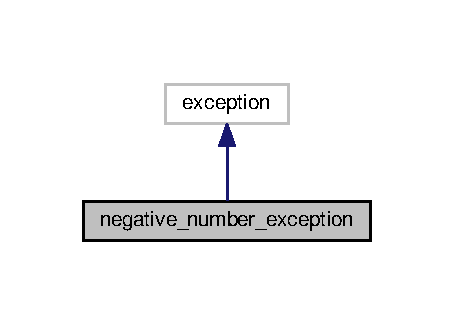
\includegraphics[width=218pt]{classnegative__number__exception__inherit__graph}
\end{center}
\end{figure}


Collaboration diagram for negative\+\_\+number\+\_\+exception\+:\nopagebreak
\begin{figure}[H]
\begin{center}
\leavevmode
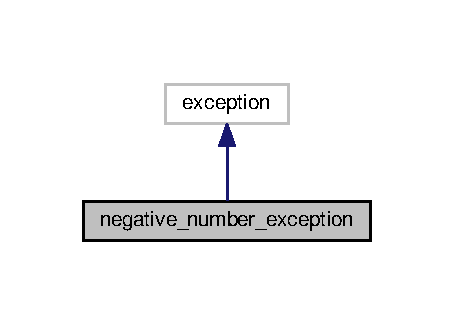
\includegraphics[width=218pt]{classnegative__number__exception__coll__graph}
\end{center}
\end{figure}
\subsection*{Public Member Functions}
\begin{DoxyCompactItemize}
\item 
virtual const char $\ast$ \hyperlink{classnegative__number__exception_aebdf986059ad346afd1e080947a115f8}{what} () const   throw ()
\begin{DoxyCompactList}\small\item\em Details the problem which invokes the exception. \end{DoxyCompactList}\end{DoxyCompactItemize}
\subsection*{Public Attributes}
\begin{DoxyCompactItemize}
\item 
\hypertarget{classnegative__number__exception_ab7f43fee2224bf3dec353fe4a98a8a26}{}int \hyperlink{classnegative__number__exception_ab7f43fee2224bf3dec353fe4a98a8a26}{value}\label{classnegative__number__exception_ab7f43fee2224bf3dec353fe4a98a8a26}

\begin{DoxyCompactList}\small\item\em Used to store the negative number which invoked the exception. \end{DoxyCompactList}\end{DoxyCompactItemize}


\subsection{Detailed Description}
Exception invoked by negative numbers. 

This exception can be used when a negative number is used, where it is not suited. 

\subsection{Member Function Documentation}
\hypertarget{classnegative__number__exception_aebdf986059ad346afd1e080947a115f8}{}\index{negative\+\_\+number\+\_\+exception@{negative\+\_\+number\+\_\+exception}!what@{what}}
\index{what@{what}!negative\+\_\+number\+\_\+exception@{negative\+\_\+number\+\_\+exception}}
\subsubsection[{what}]{\setlength{\rightskip}{0pt plus 5cm}const char $\ast$ negative\+\_\+number\+\_\+exception\+::what (
\begin{DoxyParamCaption}
{}
\end{DoxyParamCaption}
) const throw  ) \hspace{0.3cm}{\ttfamily [virtual]}}\label{classnegative__number__exception_aebdf986059ad346afd1e080947a115f8}


Details the problem which invokes the exception. 

\begin{DoxyReturn}{Returns}
A string detailing the exception 
\end{DoxyReturn}


The documentation for this class was generated from the following files\+:\begin{DoxyCompactItemize}
\item 
/home/adamleon/code\+\_\+quality/code\+\_\+quality\+\_\+godlike/include/\hyperlink{exceptions_8hpp}{exceptions.\+hpp}\item 
/home/adamleon/code\+\_\+quality/code\+\_\+quality\+\_\+godlike/src/exceptions.\+cpp\end{DoxyCompactItemize}

\hypertarget{classoverflow__exception}{}\section{overflow\+\_\+exception Class Reference}
\label{classoverflow__exception}\index{overflow\+\_\+exception@{overflow\+\_\+exception}}


Exception invoked by integer overflow.  




{\ttfamily \#include $<$exceptions.\+hpp$>$}



Inheritance diagram for overflow\+\_\+exception\+:\nopagebreak
\begin{figure}[H]
\begin{center}
\leavevmode
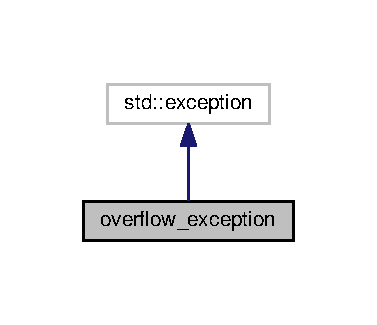
\includegraphics[width=181pt]{classoverflow__exception__inherit__graph}
\end{center}
\end{figure}


Collaboration diagram for overflow\+\_\+exception\+:\nopagebreak
\begin{figure}[H]
\begin{center}
\leavevmode
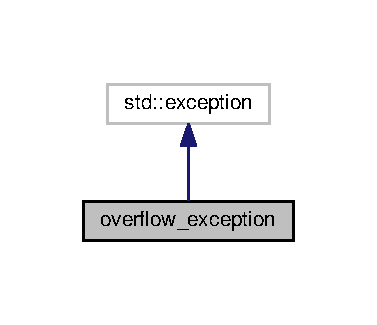
\includegraphics[width=181pt]{classoverflow__exception__coll__graph}
\end{center}
\end{figure}


\subsection{Detailed Description}
Exception invoked by integer overflow. 

This exception can be used when a number is too large. 

The documentation for this class was generated from the following files\+:\begin{DoxyCompactItemize}
\item 
/home/adamleon/code\+\_\+quality/code\+\_\+quality\+\_\+godlike/include/\hyperlink{exceptions_8hpp}{exceptions.\+hpp}\item 
/home/adamleon/code\+\_\+quality/code\+\_\+quality\+\_\+godlike/src/exceptions.\+cpp\end{DoxyCompactItemize}

\chapter{File Documentation}
\hypertarget{code__quality__godlike_8cpp}{}\section{/home/adamleon/code\+\_\+quality/code\+\_\+quality\+\_\+godlike/code\+\_\+quality\+\_\+godlike.cpp File Reference}
\label{code__quality__godlike_8cpp}\index{/home/adamleon/code\+\_\+quality/code\+\_\+quality\+\_\+godlike/code\+\_\+quality\+\_\+godlike.\+cpp@{/home/adamleon/code\+\_\+quality/code\+\_\+quality\+\_\+godlike/code\+\_\+quality\+\_\+godlike.\+cpp}}
{\ttfamily \#include $<$iostream$>$}\\*
{\ttfamily \#include \char`\"{}include/calculations.\+hpp\char`\"{}}\\*
Include dependency graph for code\+\_\+quality\+\_\+godlike.\+cpp\+:\nopagebreak
\begin{figure}[H]
\begin{center}
\leavevmode
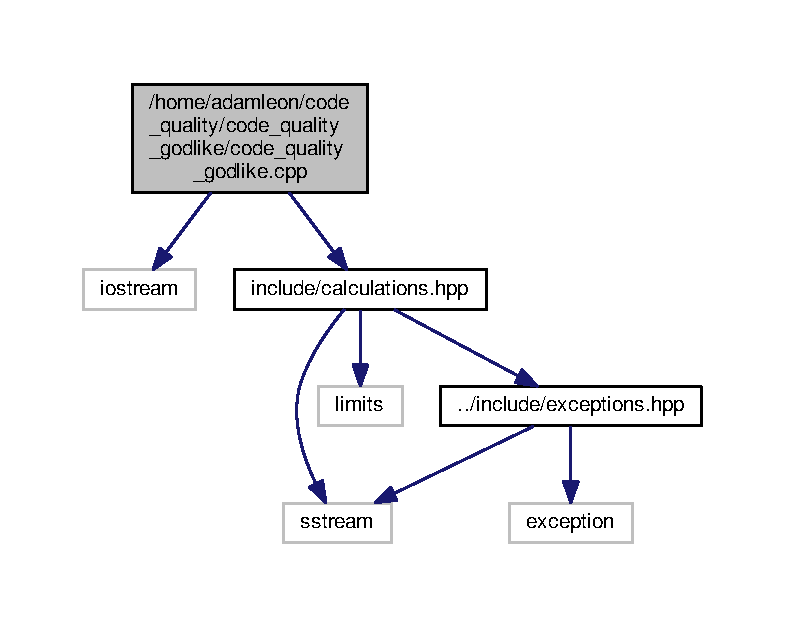
\includegraphics[width=350pt]{code__quality__godlike_8cpp__incl}
\end{center}
\end{figure}
\subsection*{Functions}
\begin{DoxyCompactItemize}
\item 
int \hyperlink{code__quality__godlike_8cpp_a0ddf1224851353fc92bfbff6f499fa97}{main} (int argc, char $\ast$argv\mbox{[}$\,$\mbox{]})
\begin{DoxyCompactList}\small\item\em Main function. \end{DoxyCompactList}\end{DoxyCompactItemize}


\subsection{Detailed Description}
\begin{DoxyAuthor}{Author}
Adam Leon Kleppe 
\end{DoxyAuthor}


\subsection{Function Documentation}
\hypertarget{code__quality__godlike_8cpp_a0ddf1224851353fc92bfbff6f499fa97}{}\index{code\+\_\+quality\+\_\+godlike.\+cpp@{code\+\_\+quality\+\_\+godlike.\+cpp}!main@{main}}
\index{main@{main}!code\+\_\+quality\+\_\+godlike.\+cpp@{code\+\_\+quality\+\_\+godlike.\+cpp}}
\subsubsection[{main}]{\setlength{\rightskip}{0pt plus 5cm}int main (
\begin{DoxyParamCaption}
\item[{int}]{argc, }
\item[{char $\ast$}]{argv\mbox{[}$\,$\mbox{]}}
\end{DoxyParamCaption}
)}\label{code__quality__godlike_8cpp_a0ddf1224851353fc92bfbff6f499fa97}


Main function. 

Takes in two arguments which are numbers a and b, and outputs the result of the equation a! + b. 
\begin{DoxyParams}{Parameters}
{\em argc} & The number of arguments \\
\hline
{\em argv} & Array containing all the arguments. \\
\hline
\end{DoxyParams}
\begin{DoxyReturn}{Returns}
0 if the computation was successful, and -\/1 if it failed. 
\end{DoxyReturn}

\hypertarget{calculations_8hpp}{}\section{/home/adamleon/code\+\_\+quality/code\+\_\+quality\+\_\+godlike/include/calculations.hpp File Reference}
\label{calculations_8hpp}\index{/home/adamleon/code\+\_\+quality/code\+\_\+quality\+\_\+godlike/include/calculations.\+hpp@{/home/adamleon/code\+\_\+quality/code\+\_\+quality\+\_\+godlike/include/calculations.\+hpp}}


This file contains global functions for the Calculation library.  


{\ttfamily \#include $<$sstream$>$}\\*
{\ttfamily \#include $<$limits$>$}\\*
{\ttfamily \#include \char`\"{}../include/exceptions.\+hpp\char`\"{}}\\*
Include dependency graph for calculations.\+hpp\+:\nopagebreak
\begin{figure}[H]
\begin{center}
\leavevmode
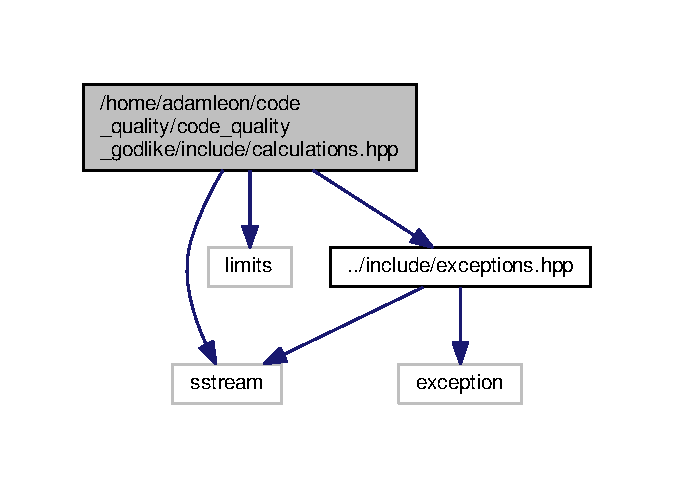
\includegraphics[width=324pt]{calculations_8hpp__incl}
\end{center}
\end{figure}
This graph shows which files directly or indirectly include this file\+:\nopagebreak
\begin{figure}[H]
\begin{center}
\leavevmode
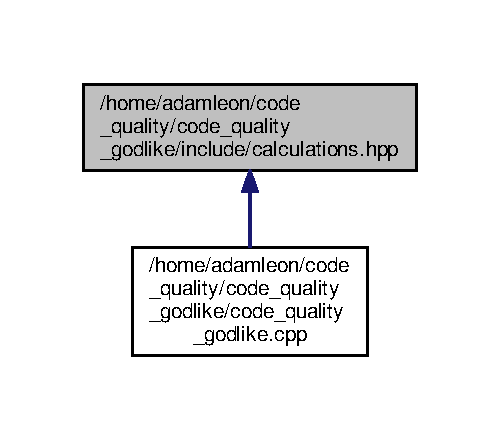
\includegraphics[width=240pt]{calculations_8hpp__dep__incl}
\end{center}
\end{figure}
\subsection*{Functions}
\begin{DoxyCompactItemize}
\item 
void \hyperlink{calculations_8hpp_a4c4dff898dfea5c7f94b17847e9ade8a}{argument\+To\+Integer} (char $\ast$argument, int \&number)
\begin{DoxyCompactList}\small\item\em Function converting a string to an integer. \end{DoxyCompactList}\item 
int \hyperlink{calculations_8hpp_af9f70ede9e2b2d55a963d27cbdb8346b}{calculate} (int a, int b)
\begin{DoxyCompactList}\small\item\em Calculates a!+b. \end{DoxyCompactList}\end{DoxyCompactItemize}


\subsection{Detailed Description}
This file contains global functions for the Calculation library. 

\begin{DoxyAuthor}{Author}
Adam Leon Kleppe 
\end{DoxyAuthor}


\subsection{Function Documentation}
\hypertarget{calculations_8hpp_a4c4dff898dfea5c7f94b17847e9ade8a}{}\index{calculations.\+hpp@{calculations.\+hpp}!argument\+To\+Integer@{argument\+To\+Integer}}
\index{argument\+To\+Integer@{argument\+To\+Integer}!calculations.\+hpp@{calculations.\+hpp}}
\subsubsection[{argument\+To\+Integer}]{\setlength{\rightskip}{0pt plus 5cm}void argument\+To\+Integer (
\begin{DoxyParamCaption}
\item[{char $\ast$}]{argument, }
\item[{int \&}]{number}
\end{DoxyParamCaption}
)}\label{calculations_8hpp_a4c4dff898dfea5c7f94b17847e9ade8a}


Function converting a string to an integer. 

Converts a string opf any length to an integer if the string represents a valid integer. 
\begin{DoxyExceptions}{Exceptions}
{\em argument\+\_\+invalid\+\_\+execption} & if the argument is not a valid integer. \\
\hline
\end{DoxyExceptions}

\begin{DoxyParams}{Parameters}
{\em argument} & The argument which is supposed to converted. \\
\hline
{\em number} & The output number of the conversion \\
\hline
\end{DoxyParams}
\hypertarget{calculations_8hpp_af9f70ede9e2b2d55a963d27cbdb8346b}{}\index{calculations.\+hpp@{calculations.\+hpp}!calculate@{calculate}}
\index{calculate@{calculate}!calculations.\+hpp@{calculations.\+hpp}}
\subsubsection[{calculate}]{\setlength{\rightskip}{0pt plus 5cm}int calculate (
\begin{DoxyParamCaption}
\item[{int}]{a, }
\item[{int}]{b}
\end{DoxyParamCaption}
)}\label{calculations_8hpp_af9f70ede9e2b2d55a963d27cbdb8346b}


Calculates a!+b. 

Calculates the equation a! + b 
\begin{DoxyExceptions}{Exceptions}
{\em negative\+\_\+number\+\_\+execption} & if a is negative \\
\hline
{\em overflow\+\_\+execption} & if either a or the result is larger than I\+N\+T\+\_\+\+M\+A\+X \\
\hline
\end{DoxyExceptions}

\begin{DoxyParams}{Parameters}
{\em a} & Integer which will be factorialized \\
\hline
{\em b} & Integer which will be added \\
\hline
\end{DoxyParams}
\begin{DoxyReturn}{Returns}
The result of the equation a!+b 
\end{DoxyReturn}

\hypertarget{exceptions_8hpp}{}\section{/home/adamleon/code\+\_\+quality/code\+\_\+quality\+\_\+godlike/include/exceptions.hpp File Reference}
\label{exceptions_8hpp}\index{/home/adamleon/code\+\_\+quality/code\+\_\+quality\+\_\+godlike/include/exceptions.\+hpp@{/home/adamleon/code\+\_\+quality/code\+\_\+quality\+\_\+godlike/include/exceptions.\+hpp}}


This file contains the exception classes for the Calculation library.  


{\ttfamily \#include $<$sstream$>$}\\*
{\ttfamily \#include $<$exception$>$}\\*
Include dependency graph for exceptions.\+hpp\+:\nopagebreak
\begin{figure}[H]
\begin{center}
\leavevmode
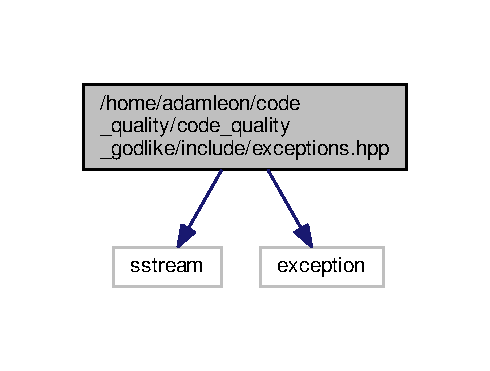
\includegraphics[width=235pt]{exceptions_8hpp__incl}
\end{center}
\end{figure}
This graph shows which files directly or indirectly include this file\+:\nopagebreak
\begin{figure}[H]
\begin{center}
\leavevmode
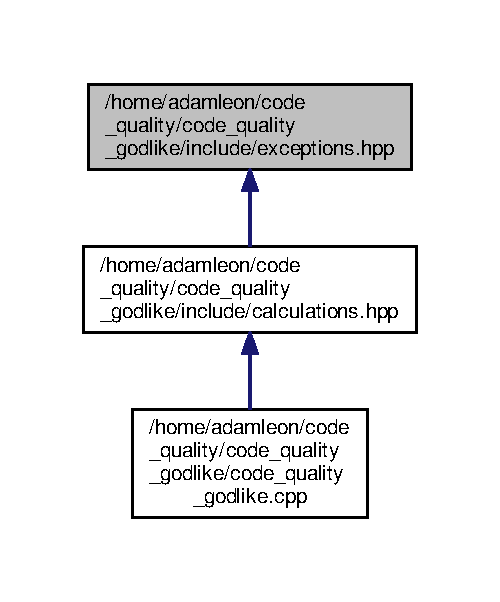
\includegraphics[width=240pt]{exceptions_8hpp__dep__incl}
\end{center}
\end{figure}
\subsection*{Classes}
\begin{DoxyCompactItemize}
\item 
class \hyperlink{classnegative__number__exception}{negative\+\_\+number\+\_\+exception}
\begin{DoxyCompactList}\small\item\em Exception invoked by negative numbers. \end{DoxyCompactList}\item 
class \hyperlink{classargument__invalid__exception}{argument\+\_\+invalid\+\_\+exception}
\begin{DoxyCompactList}\small\item\em Exception invoked by invalid arguments. \end{DoxyCompactList}\item 
class \hyperlink{classoverflow__exception}{overflow\+\_\+exception}
\begin{DoxyCompactList}\small\item\em Exception invoked by integer overflow. \end{DoxyCompactList}\end{DoxyCompactItemize}


\subsection{Detailed Description}
This file contains the exception classes for the Calculation library. 

\begin{DoxyAuthor}{Author}
Adam Leon Kleppe 
\end{DoxyAuthor}

%--- End generated contents ---

% Index
\backmatter
\newpage
\phantomsection
\clearemptydoublepage
\addcontentsline{toc}{chapter}{Index}
\printindex

\end{document}
